\documentclass{beamer}

\usepackage{graphicx}
\usepackage{amsmath}
\usepackage{verbatim}
\usepackage{relsize}
\usepackage{listings}
\usepackage{mathrsfs}


\usepackage{pgf,tikzscale,tikz}

\usetheme{Madrid}
\usecolortheme{wolverine}
\setbeamertemplate{navigation symbols}{}




\title{ Highway Games on Weakly Cyclic Graphs }
\author{Warren Keil }
%\institute{}





\begin{document}



\maketitle

\frame{\frametitle{Introduction} 
A highway problem is a problem that can be modeled with a graph such that there is a set of required paths between specific vertices. Examples of highway problems include:
\begin{itemize}
\item Choosing the locations of the construction of highways 
\item Scheduling flights between airports
\end{itemize}
}


\frame{
\includegraphics[scale=.37]{flightmap.jpg}
}

\frame{
\includegraphics[scale=.58]{road.jpg}
}

\frame{\frametitle{Definitions} 
\textbf{Cooperative Cost Game}- a pair \((N,c)\), of a set of \(N\) players and a cost function \(c\)

\vspace{4mm}
\textbf{Coalition} - is a set \(S \subset N\) of players.


\vspace{4mm}
\textbf{Minimum joint cost of \(S\)} - \(c(S)\) is the minimum cost of \(S\). 

}
\frame{\frametitle{Definition}
\textbf{Highway Problem}  \(\Gamma= (N,G,\{s_i\}_{i\in N}, \{t_i\}_{i\in N},w)  \) 

 
\begin{itemize}
\item \(N = \{1,2,\ldots, n\}\) - the indexing set of players
\item  \(G=(V,E)\) - a graph 
\item \(\{s_i\}_{i\in N}\) - the starting vertex for player \(i\)
\item \(\{t_i\}_{i\in N}\) - the terminating vertex for player \(i\)
\item  \(w: E \rightarrow \mathbb{R}_{\geq 0} \)  - a cost function that assigns a cost to each edge

\end{itemize}
}

\frame{\frametitle{Definition}
\textbf{Highway Game}  \((N, c_{\Gamma} ) \)- of a highway problem \(\Gamma\): (optimization problem)

\begin{align*}
c_{\Gamma} &= \min_{E' \subseteq E} \{w(E') | s_i \text{ and } t_i \text{ are connected in } (V,E')  \forall i \in S \}  \text{ for } S \subseteq N \}
\end{align*}
}

\frame{\frametitle{Definition}
\textbf{Weakly cyclic-} A graph \(G\) is weakly cyclic is every edge in \(G\) is contained in at most one cycle.

\textbf{Weakly triangular}- A weakly cyclic graph \(G\) is weakly triangular if every cycle in \(G\) has length 3.







\begin{center}
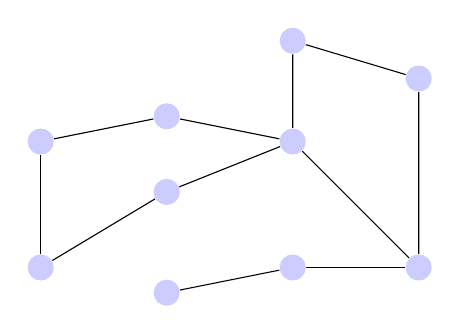
\begin{tikzpicture}
  [scale=.16,auto=left,every node/.style={circle,fill=blue!20}]
  \node (1) at (0,0) {};
  \node (2) at (0,10)  {};
  \node (3) at (10,-2)  {};
  \node (4) at (10,6)  {};
  \node (5) at (10,12)  {};
  \node (6) at (20,0)  {};
  \node (7) at (20,10)  {};
  \node (8) at (20,18)  {};
  \node (9) at (30,0)  {};
  \node (10) at (30,15)  {};


  \foreach \from/\to in {2/5,2/1,1/4,4/7,5/7,7/8,8/10,10/9,7/9,6/9,3/6}
    \draw (\from) -- (\to);

\end{tikzpicture} \hspace{10mm}
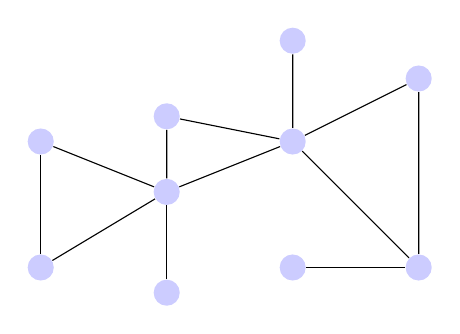
\begin{tikzpicture}
  [scale=.16,auto=left,every node/.style={circle,fill=blue!20}]
  \node (1) at (0,0) {};
  \node (2) at (0,10)  {};
  \node (3) at (10,-2)  {};
  \node (4) at (10,6)  {};
  \node (5) at (10,12)  {};
  \node (6) at (20,0)  {};
  \node (7) at (20,10)  {};
  \node (8) at (20,18)  {};
  \node (9) at (30,0)  {};
  \node (10) at (30,15)  {};


  \foreach \from/\to in {1/2,2/4,1/4,3/4,4/5,5/7,4/7,7/8,7/10,6/9,7/9,9/10}
    \draw (\from) -- (\to);

\end{tikzpicture}
\end{center}


 Weakly Cyclic   \hspace{ 55mm} Weakly Triangular 

}


\frame{\frametitle{Definition}
\textbf{Game Concavity-} A (cooperative cost) game \((N,c)\) is concave if 

\[
c(T \cup S) + c(T \cap S) \leq c(T) + c(S) \hspace{8mm}  \forall S,T \subseteq N
\]

\vspace{6mm} 
\textbf{Highway Game Concavity-} A graph \(G\) is \textbf{HG concave} if for every highway problem \(\Gamma= (N,G,\{s_i\}_{i\in N}, \{t_i\}_{i\in N},w)\), the corresponding highway game \((N,c_{\Gamma})\) is concave. 
}


\frame{ \frametitle{Example of Highway Game Concavity}


\begin{center}
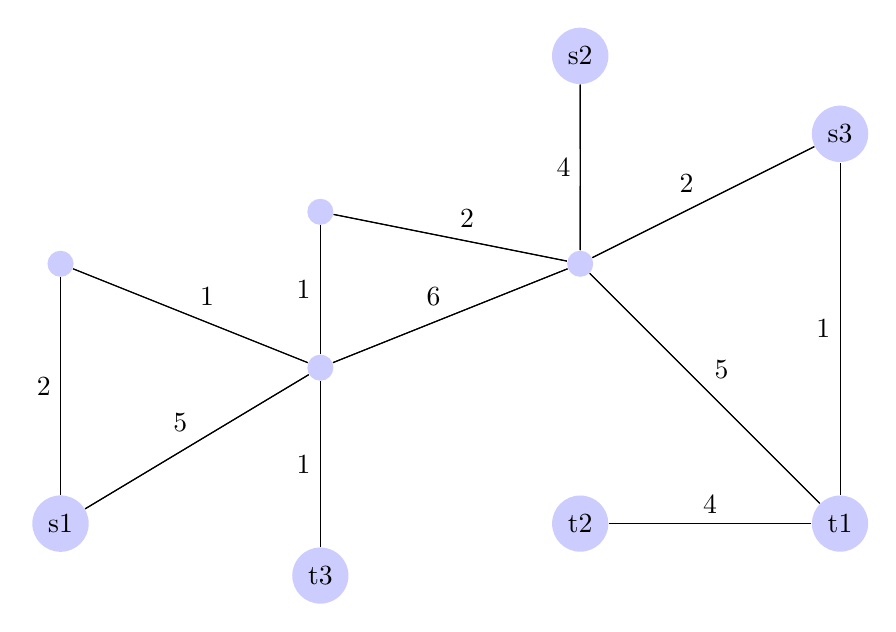
\begin{tikzpicture}
  [scale=.33,auto=left,every node/.style={circle,fill=blue!20},every edge/.append style={every node/.style={fill=white}}]
  

  \node (1) at (0,0) {s1};
  \node (2) at (0,10)  {};
  \node (3) at (10,-2)  {t3};
  \node (4) at (10,6)  {};
  \node (5) at (10,12)  {};
  \node (6) at (20,0)  {t2};
  \node (7) at (20,10)  {};
  \node (8) at (20,18)  {s2};
  \node (9) at (30,0)  {t1};
  \node (10) at (30,15)  {s3};
  

  \path[ ] (1) edge node {2} (2);
\path[ ] (2) edge node {1} (4);
\path[ ] (1) edge node {5} (4);
\path[ ] (3) edge node {1} (4);
\path[ ] (4) edge node {1} (5);
\path[ ] (5) edge node {2} (7);
\path[ ] (4) edge node {6} (7);
\path[ ] (7) edge node {4} (8);
\path[ ] (7) edge node {2} (10);
\path[ ] (6) edge node {4} (9);
\path[ ] (7) edge node {5} (9);
\path[ ] (9) edge node {1} (10);

  \foreach \from/\to in {1/2,2/4,1/4,3/4,4/5,5/7,4/7,7/8,7/10,6/9,7/9,9/10}
    \draw (\from) -- (\to);

\end{tikzpicture}
\end{center}
}

\frame{ \frametitle{Example of Highway Game Concavity}
If we have the set of players \(N=\{1,2,3\}\) and subsets \(T=\{1,3\}\) and \( S=\{2,3\} \), then notice:
\begin{align*}
c(T\cup S)&= c(\{1,2,3\}) = 2+1+1+1+2+4+2+1+4 = 18 \\
c(T \cap S) &=c(\{3\}) = 2+2+1+1 = 6 \\
c(T) &= 2+1+1+2+2+1+1 =10 \\
c(S) &= 4+2+1+4+2+1+1 = 15
\end{align*}

\[
24 = c(T\cup S) + c(T\cap S) \leq c(T) +c(S)  = 25
\]
(for this example)
}

\frame{\frametitle{Lemmas}

\textbf{Lemma 1:} Let \(\Gamma = (N,C,\{s_i\}_{i\in N},\{t_i\}_{i\in N}, w)  \) be a highway problem where \(C\) is a cycle of length 3. Then the corresponding highway game \((N,C_\Gamma)\) is concave. 

\vspace{3mm}
\textbf{Idea of Proof of Lemma 1:}
\begin{itemize}
\item For every coalition \(S\), it is optimal to either construct one or two edges.
\item If optimal to construct one edge \(\{u,v\}\) \(\Rightarrow\) \(\{s_i,t_i\} = \{u,v\} \forall i \in N\).
\item If optimal to construct two edges for a coalition then it must be optimal to construct these same.two edges for any other coalition
\end{itemize}
}


\frame{\frametitle{Lemmas}
\textbf{Lemma 2:} Let \(\Gamma = (N,G,\{s_i\}_{i\in N},\{t_i\}_{i\in N}, w)  \) be a highway problem where \(G\) is a weakly cyclic graph. Let \(\mathscr{C}(G)\) denote the set of cycles in \(G\) and \(\mathscr{BE}(G)\) denote the set of bridge edges in \(G\).   Then, 
\[
c_{\Gamma}(S) = \sum_{i\in \mathscr{C}(G) } c_{\Gamma^i}(S) + \sum_{j\in \mathscr{BE}(G) } c_{\Gamma^j}(S)  \hspace{2mm} \text{for every }S\subseteq N
\]

\textbf{Proof:} Straightforward.
}


\frame{\frametitle{Theorem 1}
\textbf{Theorem 1:} A connected graph \(G\) is HG-concave if and only if it is weakly triangular.  

\textbf{Proof.} [\(\Leftarrow\)] Suppose \(G\) is weakly triangular. Then \(G\) can be deconstructed as a bunch of bridge edges and cycles of length 3. Lemma 1 guarantees that every cycle of length 3 is HG-concave. It is trivially shown that every tree graph is HG concave and thus, every bridge edge is concave. Lemma 2 shows that the cost of any coalition of a weakly cyclic graph is equal to the sum of the costs of its individual cycles and bridge edges. Thus, \(G\) must be HG concave since it is a linear combination of HG concave graphs. 
}


\frame{\frametitle{Theorem 1}
\textbf{Proof continued.} [\(\Rightarrow\)] Suppose \(G\) is not weakly triangular. Then there exists a cycle in of length \(k\) such that \(k\geq 4\). Let, 
\[ w(e) = 
\begin{cases} 
      2 & \text{ if } e \in \{ \{v_1,v_2\}, \{v_2,v_3\} \} \\
      0 &  \text{ if } e \in \{ \{v_3,v_4\},\ldots, \{v_{k-2},v_{k-1}\} \} \\
      3 &  \text{ if } e \in \{ \{v_k,v_1\},\ldots, \{v_k,v_{k-1}\} \} \\
      100 & \text{ if } e \not \in C_k
   \end{cases}
\]

}





\frame{\frametitle{Theorem 1}
\textbf{Proof continued.} [\(\Rightarrow\)] \(N=\{1,2,3\}\). Let \(S=\{1,2\}\) and \(T=\{1,3\}\). 

\begin{center}
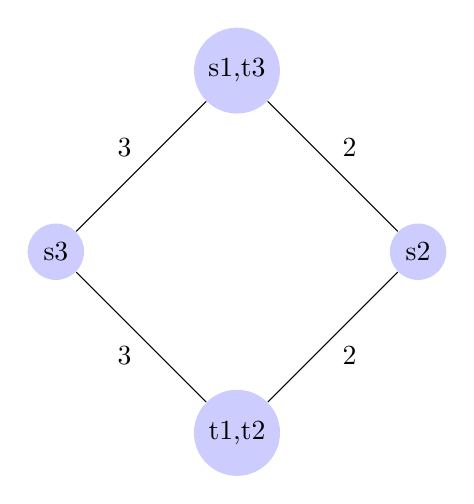
\begin{tikzpicture}
  [scale=.23,auto=left,every node/.style={circle,fill=blue!20},every edge/.append style={every node/.style={fill=white}}]
  

  \node (1) at (0,20) {s1,t3};
  \node (2) at (10,10)  {s2};
  \node (3) at (0,0)  {t1,t2};
  \node (4) at (-10,10)  {s3};
  

  \path[ ] (1) edge node {2} (2);
\path[ ] (2) edge node {2} (3);
\path[ ] (3) edge node {3} (4);
\path[ ] (4) edge node {3} (1);

  \foreach \from/\to in {}
    \draw (\from) -- (\to);

\end{tikzpicture}
\end{center}

}

\frame{\frametitle{Theorem 1}
\textbf{Proof continued.} [\(\Rightarrow\)] 
\begin{align*}
c_{\Gamma}(S) &= c_{\Gamma}(\{ 1,2 \}) =4 \\
c_{\Gamma}(T) &= c_{\Gamma}(\{ 1,3 \}) =4 \\
c_{\Gamma}(S\cup T) &=c_{\Gamma}(\{  1,2,3\}) = 7 \\
c_{\Gamma}(S\cap T) &= c_{\Gamma}(\{ 1 \}) =4
\end{align*}

\[
\Rightarrow  11 = c_{\Gamma}(S\cup T) +c_{\Gamma}(S\cap T) > c_{\Gamma}(S)+c_{\Gamma}(T)  = 8 
\]
\[
\therefore \text{ G is not HG concave } \blacksquare
\] 
}


\frame{\frametitle{Implications of Theorem 1}
This theorem can be used to:
\begin{itemize}
\item  Guarantee optimality of algorithms
\item Help determine the complexity of algorithms
\item Use in further study of properties of weakly cyclic graphs and/or HG concave graphs
\end{itemize}

}


\frame{\frametitle{Relation to Lecture}
\begin{itemize}
\item Approaches the problem by breaking graph down into smaller induced subgraphs
\item Greatly utilizes idea and properties of paths and cycles in proof
\item Uses properties of trees in proof
\item Optimization problem, similar to lots of other problems we have discussed in class.  
\end{itemize}
}

\frame{\frametitle{Reference}
\begin{thebibliography}{9}
\bibitem{latexcompanion} 
Baris Ciftci, Peter Borm, Herbert Hamers. 
\textit{Highway Games on Weakly Cyclic Graphs}. 2009.
\textit{Stochastics and Statistics}.
Elsevier. European Journal of Operational Research
\end{thebibliography}
 }

\end{document}












